% ----------------------------------------------------------------
\chapter{Evaluation}
% ----------------------------------------------------------------

Folgendes Kapitel hat zum Ziel die erarbeiteten Resulate kritisch zu bewerten. Dazu werden zunächst die Ergebnisse kurz zusammengefasst. Anschliessend wird anhand der zu Beginn definierten Anforderungen eine Gap-Analyse gemacht. Ein Experten-Workshop und eine SWOT-Analyse liefern neben weiteren Rückmeldungen auch Verbesserungen und Potential für eine Weiterentwicklung. Zum Schluss folgen erwähnenswerte Punkte, welche es zu beachten gilt, falls dieser Prototyp oder eine ähnliche Lösung für den Praxiseinsatz entwickelt wird.


\begin{figure}[htbp]
    \centering
    \begin{subfigure}[b]{0.8\textwidth}
    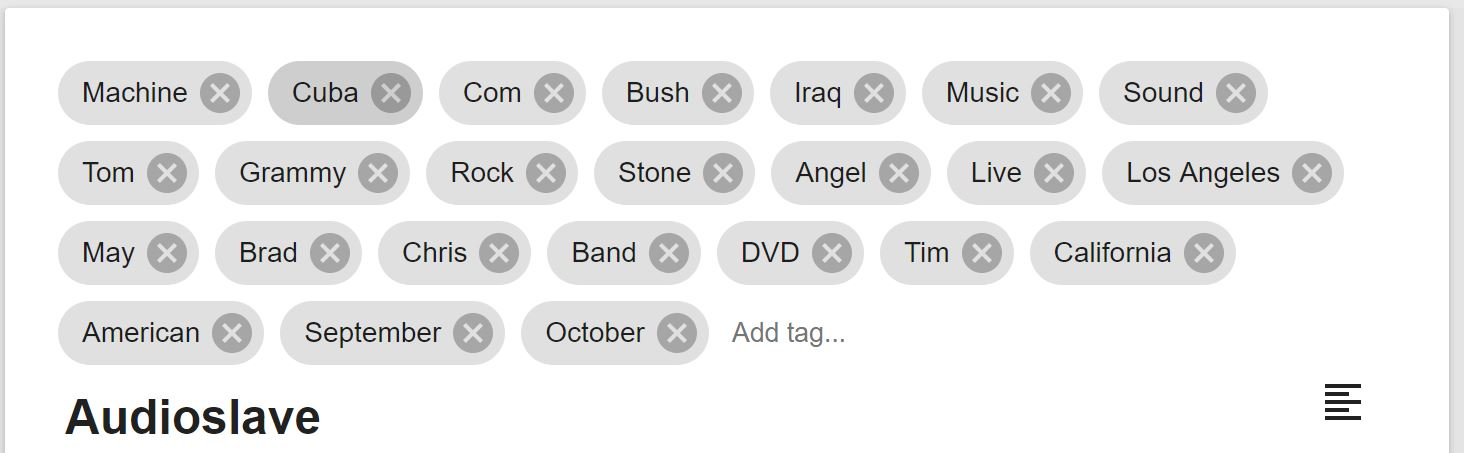
\includegraphics[width=1\linewidth]{Audioslave}
    \end{subfigure}
     \begin{subfigure}[b]{0.8\textwidth}
    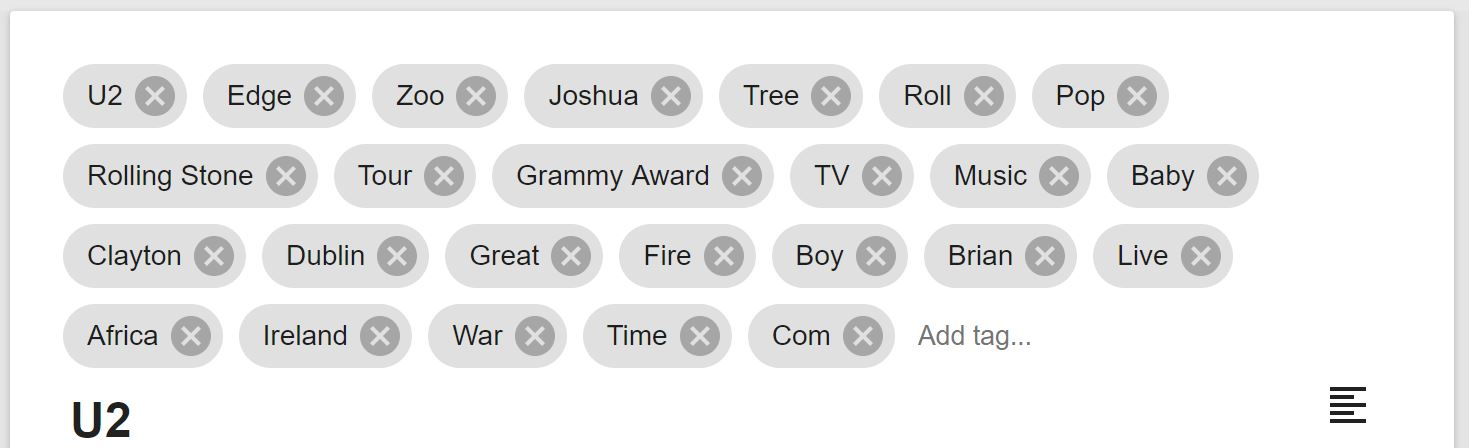
\includegraphics[width=1\linewidth]{U2}
    \end{subfigure}
     \begin{subfigure}[b]{0.8\textwidth}
    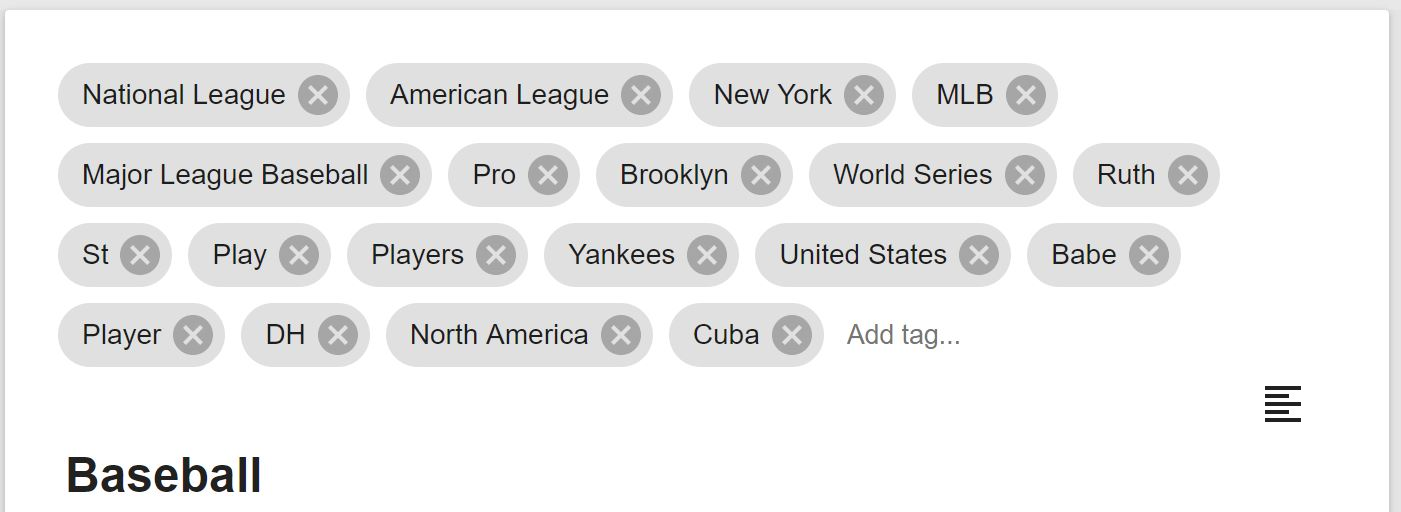
\includegraphics[width=1\linewidth]{Baseball}
    \end{subfigure}
    \caption{Keyphrase Extraktion Schwellwert}
    \label{examples-keyphrase}
\end{figure}


\section{Ergebnisse}

Der resultierende Prototyp ist in der Lage \gls{Keyphrase}[s] der Länge eins bis drei aus verschiedenen Dokumenten basierend auf einem Korpus zu extrahieren. Ebenfalls besteht die Möglichkeit, die zu einer \gls{Keyphrase} zugehörigen Dokumente zu extrahieren. \autoref{examples-keyphrase} zeigen verschiedene Beispiele von extrahierten \gls{Keyphrase}[s], dabei ist es möglich, diese in drei Gruppen zu einzuteilen:
\begin{enumerate}
    \item \textbf{Spezifische Keyphrases}, wie zum Beispiel eine Songtitel oder eine Abkürzung, haben eine sehr starke Kopplung mit dem jeweiligen Dokument. Je nach Korpus eignen sie sich sehr gut für eine Generalisierung. Jedoch können sie auch zu spezifisch sein und sind in zu wenigen Dokumenten enthalten, um Verknüpfungen automatisch zu erkennen. \textit{Bono} als Künstlername ist je nach Situation sinnvoll oder auch nicht.
    \item \textbf{Generelle Keyphrases} sind ideal für die Generalisierung. Auch wenn sie spezifisch für das jeweilige Dokument sind, tauchen sie in ausreichend vielen anderen Dokumenten auf, um dadurch Verknüpfungen aufzeigen zu können. So zum Beispiel \textit{Pop} als Musikrichtung.
    \item \textbf{Irrelevante Keyphrases} entstehen häufig durch \gls{Keyphrase}[s] der Länge vier und mehr. Sie werden nicht durch den Algorithmus abgedeckt, jedoch stückweise interpretiert. So zum Beispiel \textit{100 Greatest Artist}, welches der \gls{Keyphrase} \textit{100 Greatest Artists of All Time} entstammt.
\end{enumerate}



\subsection{Normalisierung}
Die Extraktion von relevanten \gls{Keyphrase}[s] und die entsprechende Normalisierung stellen eine grosse Herausforderung dar. Besonders, weil eine Normalisierung auf mehreren Ebenen benötigt wird:
\begin{itemize}
    \item \textbf{Korpus-Ebene}: Der Korpus wächst und verändert sich mit der Zeit. Die Relevanz der \gls{Keyphrase}[s] kann sich daher über die Zeit ebenfalls ändern. Daher gibt es die Möglichkeit \gls{Keyphrase}[s] verschiedener Korpus-Grössen miteinander zu vergleichen.
    \item \textbf{Dokument-Ebene}: Innerhalb eines Dokuments ist es wichtig, gleiche \gls{Keyphrase}[s] verschiedener Dokumente unterschiedlicher Längen vergleichen zu können. Daher sollte die Relevanz einer \gls{Keyphrase} pro Dokument normalisiert werden.
    \item \textbf{Text-Ebene}: Ebenfalls ist die Verteilung einer \gls{Keyphrase}[s] innerhalb eines Dokumentes ist eine wichtige Metrik. Gewisse Wörter tauchen nur zu Beginn oder am Schluss auf, während andere gleichmässig über den ganzen Text verteilt sind. Durch die Normalisierung dieser Metrik wären Vergleiche auf dieser Ebene möglich.
    \item \textbf{Keyphrase-Ebene}: Je länger ein \gls{Keyphrase} ist umso mehr unterscheidet sich auch der entsprechende Relevanz-Score. Tendenziell haben längere \gls{Keyphrase} einen höheren \gls{Score} als kürzere. Besonders bei der Extraktion von sowohl relevanten aber auch zum Teil generellen \gls{Keyphrase}[s] ist die Normalisierung wichtig, um verschiedene Längen vergleichen zu können.
\end{itemize}

Innerhalb des Prototypen wurde nur aufgrund der Länge eines einzelnen Dokuments normalisiert. Jedoch kann im \gls{ikc-core} sowohl der Schwellenwert als auch eine untere Limite der Anzahl Dokumente, welche die jeweilige \gls{Keyphrase}[s] enthalten, definiert werden. \autoref{threshold} zeigt als Beispiel, welche Auswirkungen die Anpassung des Schwellenwerts auf die Anzahl \gls{Keyphrase}[es] hat. Während \autoref{minidoc} die Auswirkung der Erhöhung der unteren Limite der verschiedenen Dokumenten pro \gls{Keyphrase} aufzeigt. Die beiden werden idealerweise miteinander kombiniert.

\begin{figure}[H]
    \centering
    \begin{subfigure}[b]{0.8\textwidth}
    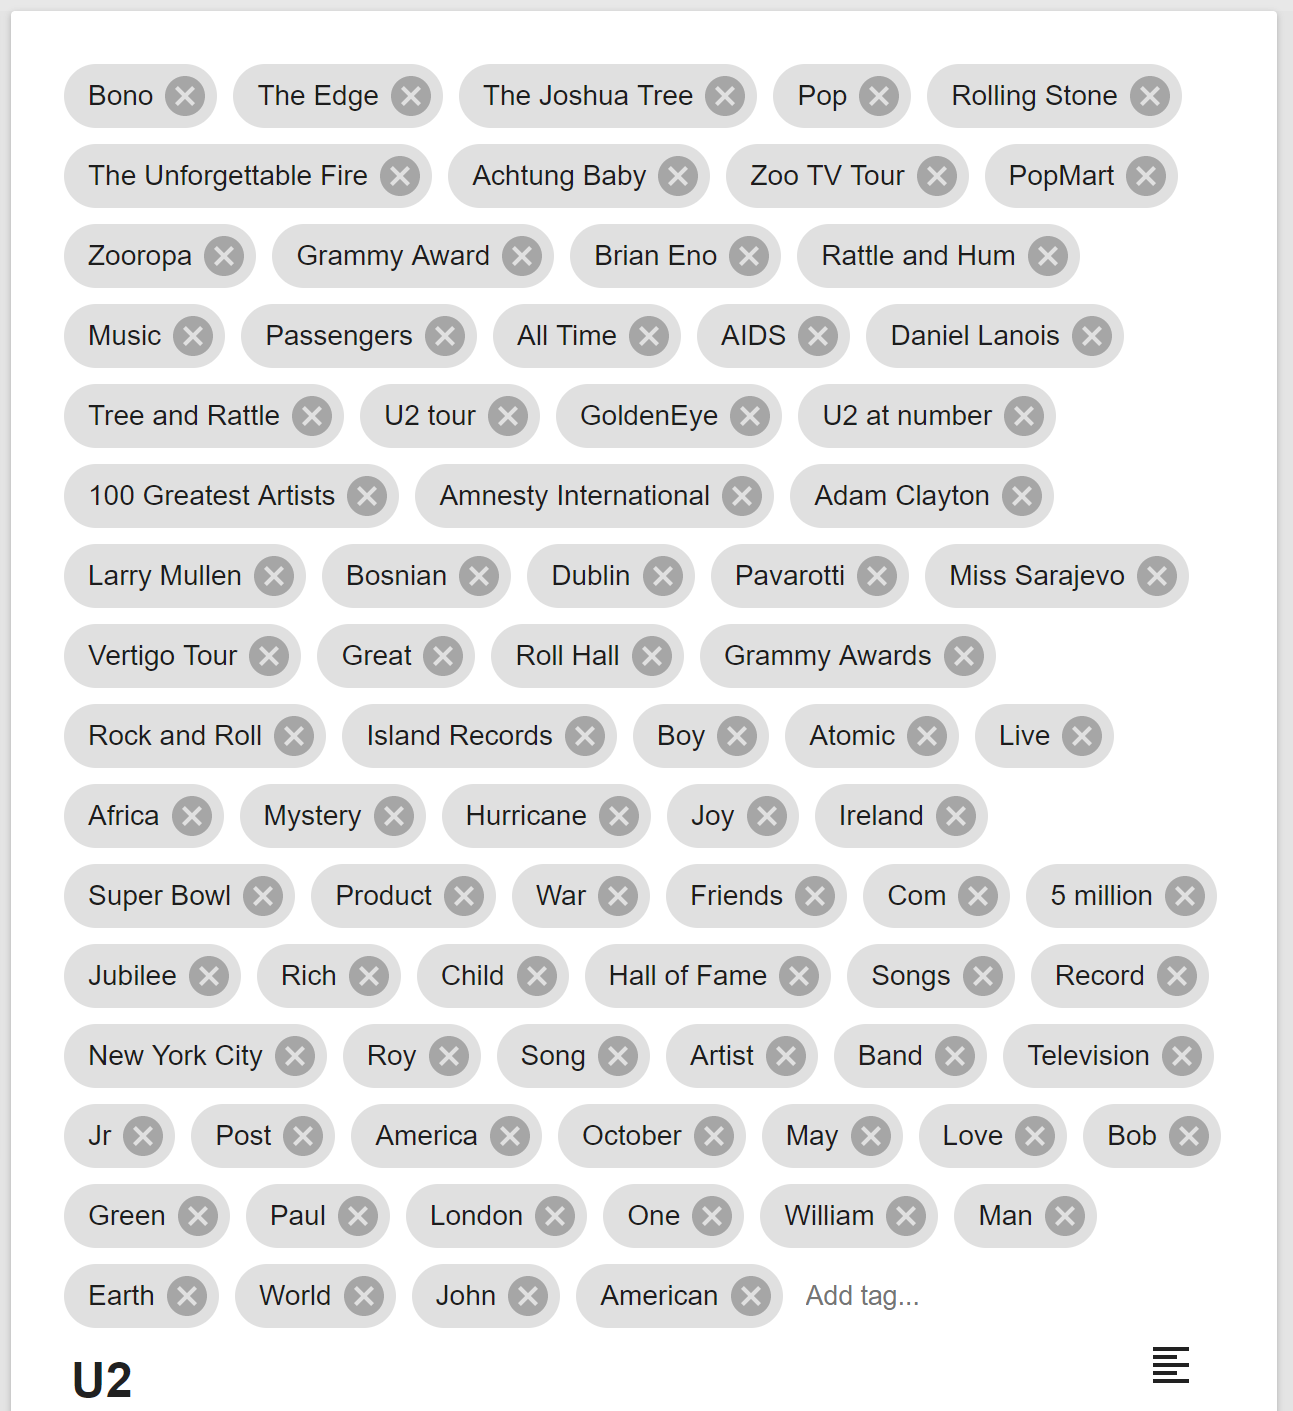
\includegraphics[width=1\linewidth]{Keyphrase-3}
    \caption{Schwellwert 0.0}
    \end{subfigure}
     \begin{subfigure}[b]{0.8\textwidth}
    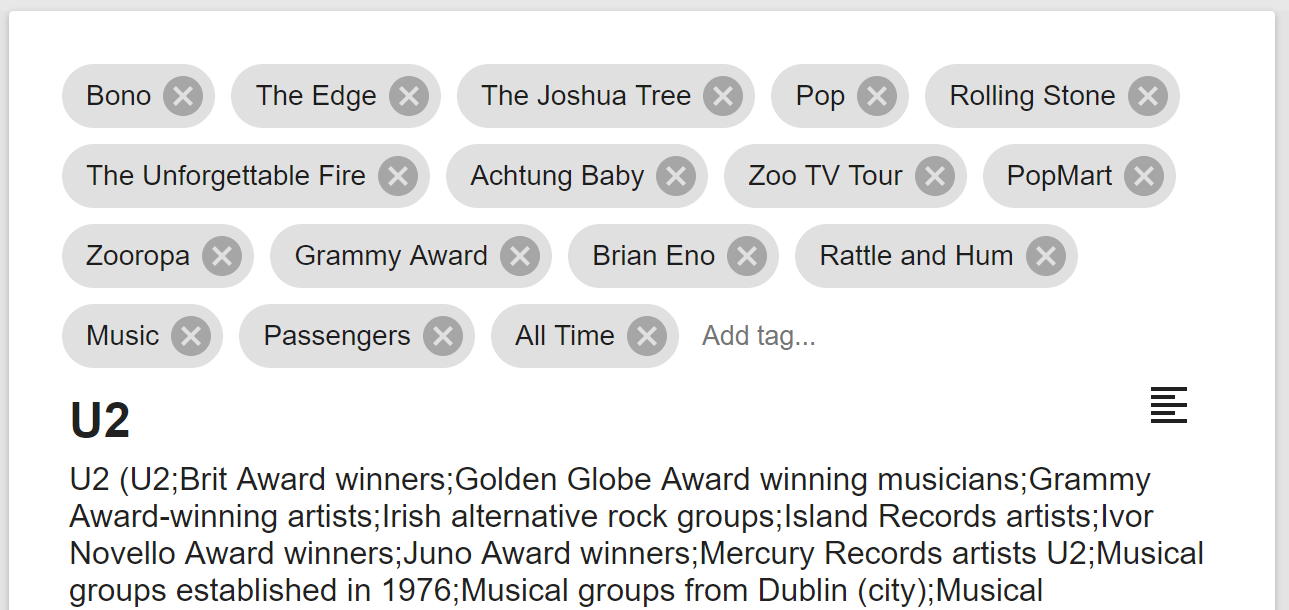
\includegraphics[width=1\linewidth]{Keyphrase-1}
    \caption{Schwellwert 0.04}
    \end{subfigure}
     \begin{subfigure}[b]{0.8\textwidth}
    
\includegraphics[width=1\linewidth]{Keyphrase-2}
    \caption{Schwellwert 0.1}
    \end{subfigure}
    \caption{Keyphrase Extraktion Schwellwert}
    \label{threshold}
\end{figure}

\begin{figure}[H]
    \centering
    \begin{subfigure}[b]{0.8\textwidth}
    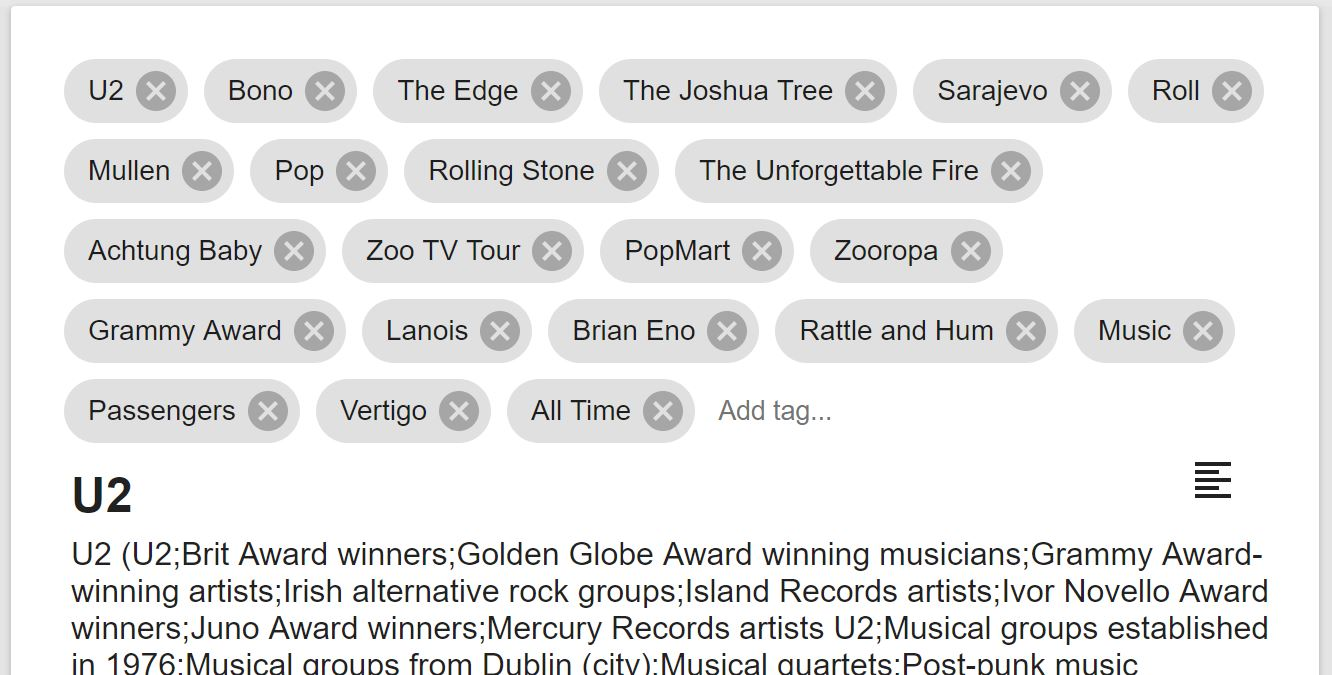
\includegraphics[width=1\linewidth]{MinDoc-0}
    \caption{Limite 0}
    \end{subfigure}
    \begin{subfigure}[b]{0.8\textwidth}
    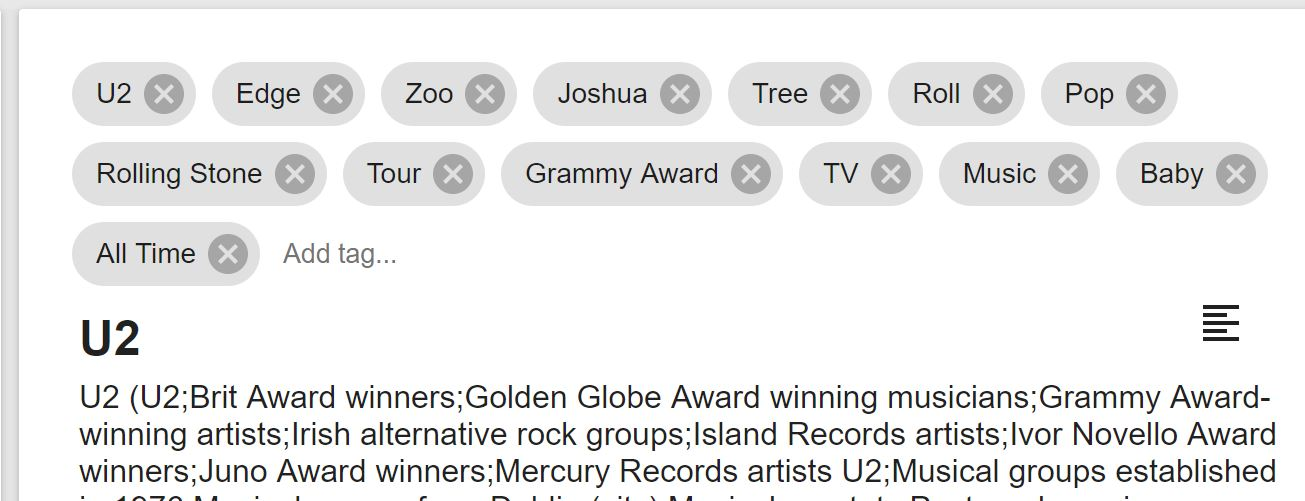
\includegraphics[width=1\linewidth]{MinDoc-10}
    \caption{Limite 10}
    \end{subfigure}
    \begin{subfigure}[b]{0.8\textwidth}
    
\includegraphics[width=1\linewidth]{MinDoc-50}
    \caption{Limite 50}
    \end{subfigure}
    \begin{subfigure}[b]{0.8\textwidth}
    
\includegraphics[width=1\linewidth]{MinDoc-100}
    \caption{Limite 100}
    \end{subfigure}
    \caption{Keyphrase Extraktion Minimum Dokuments}
    \label{minidoc}
\end{figure}



\subsection{Vergleich MoreLikeThis}
\textit{MoreLikeThis} (MLT) ist eine Funkion aus der \textit{Lucene}-Bibliothek. Sie liefert relevante Wörter eines Textes, diese dienen einem Vergleich mit den im Projekt erhaltenen Resultate. Dabei fallen einige Unterschiede auf: Während \textit{MLT} auf Wörter beschränkt ist, liefert der Prototyp \gls{Keyphrase}[s] bis zur Länge drei. Jedoch sind die Wörter aus \textit{MLT} im Schnitt genereller als die resultierenden \gls{Keyphrase}[s] des Prototypen. Dafür sind die \gls{Keyphrase}[s] zum grössten Teil bereinigt von Duplikaten (z.b. \textit{band} und \textit{band\grq s}). Ein Vergleich dieser Art ist sehr wertvoll. Auf eine vertiefte Analyse der Ergebnisse auf dieser Basis musste aus Zeitgründen verzichtet werden.
% ----------------------------------------------------------------
\section{Soll-Ist Vergleich}
% ----------------------------------------------------------------

Durch einen Soll-Ist Vergleich anhand der definierten Anforderungen (\autoref{sec:anforderungen}) kann eine erste qualitative Evalutation vorgenommen werden. Die beiden Tabellen (\autoref{tab:funktionale-anforderungen-eval}, \autoref{tab:nicht-funktionale-anforderungen-eval}) geben eine Überblick über den Stand der Anforderungen. Wie zu sehen sind bis auf zwei Ausnahmen alle Anforderungen erfüllt. 

Aufgrund des beschränkten Zeitrahmens und des agilen Projektmanagements wurde bewusst auf die Umsetzung dieser beiden Anforderungen verzichtet. Da die Datenquelle und Persistenzbasis mittels \gls{SFTP} bereits vollständig implementiert ist, ist die Anbindung eines weiteren Dienstes lediglich eine Frage der Zeit. Die Schnittstellen sind definiert und damit sind die Grundlagen gewährleistet. Die Anbindung einer weiteren Datenquelle bringt im Projektrahmen keinen eigentlichen Mehrwert, da der Fokus klar auf der Volltextsuche und der \gls{Keyphrase}-Extraktion liegt.

Auf einen Teil der Anforderungen wurde ein besonderes Augenmerk gelegt. Diese Anforderungen sind in der nachfolgenden Aufstellung kurz mit den entsprechenden Gründen zusammengefasst.

\begin{itemize}
    \item Die hohe Entkopplung zwischen den verschiedenen Klassen, Komponenten und Services ist ein wichtiger Architekturtreiber und gleichzeitig auch ein Teil der Ziele. Das Projekt dient in Zukunft als Basis für weitere Projekte, darum ist eine Wie\-der\-ver\-wend\-bar\-keit und eine leichte Erweiterbarkeit zentral. Während der Entwicklung hat sich weiter bewahrheitet, dass dies essentielle Bedingungen für eine erfolgreiche Entwicklung sind.
    \item In den Algorithmus wurde viel Zeit investiert. Dank dem bereits vorhandenem Wissen und diversen angeregten Diskussionen konnte das Projekt insbesondere auch im Bereich des Algorithmus enorm vorangetrieben werden. Dadurch konnte die anfänglich funktionierende Implementation bis in eine unerwartete technische Tiefe ausgearbeitet werden. Die solide Grundlage für zukünftige Forschung besteht.
    \item Die Anforderung A11 erwartet, dass Tags als Links dem Wissensnetzwerk hinzugefügt werden können. Der \texttt{ElementCache} ermöglicht schon in der aktuellen Version des Prototyps ein Traversieren des Wissensnetzwerks zusätzlich anhand von Tags.
    %urch die Anforderung A11 ist eine Navigation durch das Wissensnetzwerk mittels Tag-Links implizit vorausgesetzt. Zusätzlich ist es auch im Sinne des Projekts.
\end{itemize}

% Entkopplung = Architekturtreiber
% Algorithmus = Hautperformancefaktor
% A11: Im Sinne des Projektes, Resultat des agilgen Projektmanagements


% Algorithmus viel detaillierter, Mixins (zusätzlicher Aufwand für Entkopplung), Navigation über \gls{Keyphrase}[s], Recherche, 

Recherchephase


\begin{longtable}{|p{1.5cm} | p{1.5cm} | p{8.1cm}|}
  \hline
    ID & Status & Bemerkung \\\hline
    A1 & Erfüllt & Die Daten der externen Datenquelle (\gls{SFTP}) kann mittels Volltext-Index durchsucht werden.\\\hline
    A2 & Erfüllt & Das besprochene Konzept für die Autoindexierung wurde erfolgreich umgesetzt. Neue oder geänderte Dateien werden automatisch berücksichtigt.\\\hline
    A3 & Erfüllt & Der Benutzer kann seinen \gls{SFTP}-Zugang und den Pfad des zu indexierenden Ordners in der Benutzeroberfläche angeben. \\\hline
    A4 & Erfüllt & Es können sowohl alle Knoten als auch alle Dokumente externer Datenquellen durchsucht werden. \\\hline
    A5 & Erfüllt & Die Volltextsuche ist innerhalb des Suchfeldes in der bestehenden integriert. \\\hline
    A6 & Erfüllt & Die Resultate aus der externen Quelle werden optisch differenziert mit einem neuen Icon angezeigt. \\\hline
    A7 & Erfüllt & Berechnete \gls{Keyphrase}[s] zum jeweiligen Dokument auf Basis des verfügbaren Korpus werden dem Benutzer oberhalb des Titels vorgeschlagen. \\\hline
    A8 & Erfüllt & Generierte \gls{Keyphrase}[s] sind als Chip-Liste dargestellt und können bei Bedarf gelöscht werden.\\\hline
    A9 & Erfüllt & Der Benutzer kann sein Wissensnetzwerk mit Tags erweitern.\\\hline
    A10 & Erfüllt & Bereits bestehende Tags werden als Vorschlag beim Hinzufügen von neuen Tags angezeigt.\\\hline
    A11 & Erfüllt & Die Knoten und Kanten werden während der Berechnung erstellt und in einem lokalen Cache gespeichert. Bei Änderungen werden diese permanent ins Wissensnetzwerk des Benutzers übertragen.\\\hline
    A12 & Erfüllt & Tags werden als Chips dargestellt.\\\hline
    A13 & Erfüllt & \gls{N-Gramm}[s] werden ebenfalls als \gls{Keyphrase} beachtet\\\hline
    A14 & Erfüllt & In der Konfiguration kann ein beliebiger \gls{SFTP}-Server angegeben werden.  \\\hline
    \newpage
    \hline
    A15 & Hängig & \multirow{2}{8.1cm}{Sowohl die Anbindung an Dropbox und auch an Evernote wurde bewusst mit der niedrigsten Priorität versehen. Spätestens nach der detaillierten Anforderungsanalyse wurde klar entschieden, dass \gls{SFTP} als Datenquelle und Persistenz verwendet wird. Deshalb wurde auf die Umsetzung dieser beiden Anforderungen aus Zeitgründen bewusst verzichtet.}\\\cline{1-2}
    A16 & Hängig & \\[4cm]\hline
    \caption{Evaluation funktionale Anforderungen}
  \label{tab:funktionale-anforderungen-eval}
\end{longtable}


\begin{longtable}{|p{1.5cm} | p{1.5cm} | p{8.1cm}|}
  \hline
    ID & Status & Beschreibung \\\hline
    A1 & Erfüllt & Die Autoindexierung wird komplett auf dem \texttt{IndexService} ausgeführt, selbst bei einem Fehlerfall wird der Benutzer in der Nutzung des \gls{ikc-core}[s] nicht beeinträchtigt.\\\hline
    A2 & Erfüllt & Die Extraktion der \gls{Keyphrase}[s] geschieht innerhalb nützlicher Frist. Die Dauer hängt dabei von der Grösse der Datenbasis. Bei extrem grossen Datenmengen (>100k) kann dieser Prozess circa zwei Sekunden in Anspruch nehmen.\\\hline
    A3 & Erfüllt & Durch die Anbindung an den \texttt{DataService} wird die externe Datenquelle für den \gls{ikc-core} abstrahiert.\\\hline
    A4 & Erfüllt & Die zu leistenden Stunden sind abgearbeitet.\\\hline
    A5 & Erfüllt & Das Arbeitsjournal wurde entsprechend der geleisteten Stunden ausgefüllt.\\\hline
    A6 & Erfüllt & Der \gls{ikc-core} wurde in seiner Funktionalität erweitert. Auch bilden die Resultate dieser Arbeit eine gute Grundlage für weitere Forschung.\\\hline
    \caption{Evaluation funktionale Anforderungen}
  \label{tab:nicht-funktionale-anforderungen-eval}
\end{longtable}

% ----------------------------------------------------------------
\section{Experten-Workshop}
% ----------------------------------------------------------------

Ein Teil der qualitativen Evaluation ist ein Experten Workshop zu dem entstandenen Prototypen und den Resultaten dieser Arbeit. Er soll deren objektive Meinung, als auch Überlegungen zu möglichen Anwendungsfällen oder Optimierungen enthalten. Als Experten wurden Michael Kaufmann (Projektpartner) und Kevin Stadelmann (Student Wirtschaftsinformatik) ausgewählt. Da sie bereits mit den Mög\-lich\-keit\-en und der Anwendung des \gls{ikc-core}[s] vertraut sind, stellen sie ideale Teilnehmer dar. Zu Herrn Stadelmann gilt es anzumerken, dass er seine Bachelor-Arbeit ebenfalls zum Projekt \gls{IKC} verfasst. Diese beschäftigt sich insbesondere mit den wirtschaftlichen Aspekten. Zusätzlich hat er Befragungen zum Projekt durchgeführt.

Der Workshop ist in fünf Teile gegliedert:
\begin{enumerate}
    \item \textbf{Einleitung}: Im ersten Teil des Gespräches wird die Funktionalität des Prototypen kurz umschrieben. Anschliessend sollen die beiden Experten ihre Erwartungen formulieren. Dabei geht es darum, von ihnen eine Vorstellung ihrer Erwartungen unabhängig von dem resultierenden Prototypen zu erhalten. Dies ist insbesondere für die Weiterentwicklung wertvoll, sobald anstelle der Funktionalität der Benutzer in den Vordergrund rückt.
    \item \textbf{Demonstration}: Anschliessend wird den Experten der Prototyp vorgestellt. Dadurch sollen sie unsere Umsetzung und die Funktionalität genauer kennenlernen. Falls gewünscht, kann der Prototyp auch von ihnen bedient werden.
    \item \textbf{Details zur Umsetzung}: Nach der Demonstration werden einzelne Punkte der Umsetzung aber auch der Resultate genauer erläutert.
    \item \textbf{Rückmeldungen}: Nun werden Rückmeldungen, Anregungen und Kritik der Teilnehmer entgegengenommen. Diese können sowohl den Prototypen, die Resultate und auch das Projekt an sich betreffen.
    \item \textbf{Diskussion}: Die offene Diskussion zum Schluss soll als Plattform dienen um einen Schritt weiter zu denken. Dabei soll es vor allem um mögliche Anwendungen, Erweiterungen oder Anpassungen gehen.
\end{enumerate}

% ----------------------------------------------------------------
\subsection{Resultate}
% ----------------------------------------------------------------

Aus dem Workshop gingen viele interessante Resultate hervor. Die wichtigsten sind nachfolgend kurz zusammengefasst. Die Resultate sind dreigeteilt aufgeführt in Prototyp, Fragen und Unklarheiten sowie Weiterentwicklung.

\subsubsection{Prototyp}
Resultate, welche den Protypen direkt betreffen, sind hier aufgeführt.

\begin{itemize}
    \item Die automatische Kategorisierung (Tagging) von Daten wurde als sehr wertvolle Funktion genannt. Oftmals liegen viele alte, un\-struk\-tu\-rier\-te Daten vor. Die Aufbereitung dieser ist mit grossem Aufwand verbunden. Eine automatische Lösung ist darum wünsch\-ens\-wert und bedeutet einen grossen Mehrwert.
    \item Die automatische Generierung von Wissen wird allgemein als sehr wertvoll erachtet. Insbesondere dann, wenn es Mög\-lich\-ket\-en aufzeigt, welche der Benutzer selbst nicht erachtet oder erwartet hätte.
    \item Neben der automatischen Kategorisierung ist das manuelle Tagging eine weitere wichtige Funktion. Damit es einfach, beispielsweise Projektzugehörigkeiten anzugeben. Ordnung und Struktur sind so effizient und leicht zu schaffen.
    \item Die Anzahl der angezeigten Tags wurde bemängelt: Für die Benutzer ist weniger mehr. Es sollen besser wenige gute, als viele eher schlechte Tags vorgeschlagen werden. Ganz allgemein sollen Zusatzfunktionen zwar sichtbar aber nicht zu präsent in der Benutzeroberfläche sein. Beispielsweise sollen Tags und Verknüpfungen standardmässig zugeklappt / versteckt sein. So hat der Benutzer direkt einen besseren Überblick und wird gleichzeitig nicht mit Informationen überflutet.
    \item Eine Suchfunktion, welche im Volltext der verknüpften Dokumente sucht, ist das wahrscheinlich grösste Wertangebot des Prototypen. Sie ermöglicht ein effizienteres Arbeiten und spart Zeit, da schnell und einfach über alle verknüpften Datenquelle gesucht werden kann.
    \item Die Suchfunktionalität dient nicht nur dem Finden von Gesuchtem. Oftmals wird es als Navigation benutzt, indem gesucht wird, was betrachtet werden will. Ein mühselige Durchklicken wird tritt immer mehr in den Hintergrund.
\end{itemize}

\subsubsection{Fragen und Unklarheiten}
Hier sind aufgetauchte Fragen oder Unklarheiten zu finden.

\begin{itemize}
    \item Nodes und Links (Verknüpfungen) bilden die Grundlage des \gls{ikc-core}. Während der Diskussion kam die Frage nach der Differenzierung auf: Was ist ein Tag und was ist eine Verknüpfung. Im Sinne der grundlegenden Netzwerk- / Graphentheorie ist jedes Tag auch eine Verknüpfung und damit ein Teil des Wissensnetzwerks.
    \item Weiter wurde gefragt, ob für die Extraktion von \gls{Keyphrase}[s] mehrere Algorithmen genutzt werden. Wie in der Dokumentation ersichtlich, wird momentan lediglich ein Algorithmus eingesetzt. Der Prototyp ermöglicht aber das Testen von verschiedenen Varianten. So können potentielle Optionen geprüft werden. Beispielsweise könnten für verschiedene Dokumenttypen auch verschiedene Algorithmen benutzt werden, welche mit der jeweiligen Struktur umgehen können. Dieser Punkte könnte auch für Weiterentwicklung in Betracht gezogen werden.
\end{itemize}

\subsubsection{Weiterentwicklung}
Mögliche Ideen und Ansätze für die Weiterentwicklung, welche wäh\-rend des Workshops zur Sprache kamen, sind in diesem Abschnitt ersichtlich.

\begin{itemize}
    \item Die Integration der neuen Funktionen und die Benutzeroberfläche des \gls{ikc-core}[s] ganz generell (User Interface - und User Experience Design) ist benutzbar und in Ordnung. Allerdings gibt es dort sicherlich noch viel Optimierungspotential. Dies liegt in der Verantwortung von Folgeprojekten.
    \item Das automatische Tagging ist, wie gesehen, ein Wertangebot. Es gibt aber noch grossen Forschungsbedarf für einen Beweis, dass es wirklich funktioniert und auch diesen erwarteten Mehrwert bieten kann. Die Definition der Relevanz und dem Sinn (oder Unsinn) von extrahierten Inforamtionen ist nicht trivial.
    \item Ein Problem stellen wichtige Begriff dar, welche aber nur selten im Text oder Korpus auftauchen. Der Benutzer möchte diese Begriff aber inbesondere für das automatische Tagging nutzen. Ein Begriff dafür ist 'Named Entity Recognition'. Ein einfache und sehr effiziente Möglichkeit für die Umsetzung dieser Funktionalität ist die Einführung von White- beziehungsweise Blacklists. Enthält ein Dokument lediglich einmal ein Wort der Whitelist, wird es automatisch mit diesem getaggt. Die Blacklist funktioniert umgekehrt, egal wie viele Male ein Wort enthalten ist, es wird nie zum Tagging genutzt. Mit diesen Mitteln kann der Benutzer das automatisch Tagging leicht und schnell unterstützen.
    \item Die benutzerdefinierte und auch automatisch Priorisierung von Links, dem Inhalt und auch den Tags spielt eine wichtige Rolle für Benutzer. Dafür ist die Einführung eines Masses der Priorität notwendig. Eine gute Möglichkeit für Verknüpfungen und Tags wäre beispielsweise, dass die Position automatisch der Priorität entspricht. So könnte der Benutzer die Priorität selbstständig durch das Verschieben der Eigenschaft (Drag'n'Drop) festlegen.
    \item Das Konzept einer automatischen Suche mit selbstständigem Tagging treibt das Konzept der Whitelist weiter: Der Benutzer kann sein einges Regelwerk erstellen. Beispielsweise kann er mehrere Begriffe ($t_x$) zu einem Tag ($T_y$) hinterlegen: $t_1\wedge t_2 \wedge t_3 \Rightarrow T_1$ Sind diese Begriff nun in einem Dokument enthalten, wird dieses automatisch mit dem festgelegten Tag versehen. Die Konjunktion und die Disjunktion sind hier denkbar.
    Intelligente Suche: Sobald eine Menge von bestimmten Begriffen enthalten ist, wird das Dokument mit definierten Tag versehen.
    \item Die Suchfunktion steht klar im Zentrum der Weiterentwicklung. Zusatzfunktionen, wie beispielsweise die autmatische Extraktion von Informationen, können das Wertangebot aber zusätzlich erheblich steigern.
%    \item X-MAS
    \item Aus Kundensicht muss der Mehrwert eines Produkts ganz klar im Vordergrund stehen und sofort ersichtlich sein. Andernfalls wird das Interesse gar nicht erst geweckt.
    \item Schon im jetzigen Stand hat der Prototyp Zugriff auf Daten des Benutzers. Durch die Auswahl von automatisch generierten \gls{Keyphrase}[s] enthält das Wissensnetzwerk schnell ein sehr detailliertes und persönliches Abbild oder Abstraktion einer Person. Fragen des Daten- und Persönlichkeitsschutzes stehen im Raum und sind zu klären. Insbesondere die gerade aktuell in den Medien befindlichenn Änderungen sind ein kritischer Faktor für die Weiterentwicklung.
    \item Insbesondere im B2B-Kontext hat das persönliche Datenmanagement und damit der persönliche Index einen hohen Stellenwert. Denn es existieren noch keine bekannten Lösungen, welche die Bedürfnisse eines jeden Einzelnen, anstelle derjenigen der Unternehmung ihrer Gesamtheit, erfüllen. 
\end{itemize}

%klarer Usecase bzw. mehrwert
%bestehende Daten sollen möglichst ohne Aufwand indexiert werden
%Manuelles Tagging um spezifische Keyphrases zu priorisieren => Black- Whitelisting
%einzelne Keyphrases wichtigkeit z.b. häufigkeit
%Mehrere Algorithmen für unterschiedliche Resultaten
%Besser wenig Keyphrases dafür richtige 

% ----------------------------------------------------------------
\subsection{Fazit}
% ----------------------------------------------------------------

Die Resultate des Workshops sind sehr zufriedenstellend. Es wurden zahlreiche wichtige Punkte für die Weiterentwicklung gefunden. Das Wertangebot der Suche und auch der automatischen Kategorisierung ist klar ersichtlich. Der Prototyp zeigt auf, was für Möglichkeiten die \gls{Keyphrase} Extraction bietet und auch, dass es darin noch viel Potential gibt. Er ist so eine gute Grundlage für die Weiterentwicklung und auch die Forschung. Insbesondere der Algorithmus für die Bestimmung von relevanten \gls{Keyphrase}[s] bedarf noch intensiver Arbeit.

%\begin{itemize}
%    \item Nutzen für Praxis   
%\end{itemize}

% ----------------------------------------------------------------
\section{SWOT-Analyse}
% ----------------------------------------------------------------

Die SWOT-Analyse als Instrument der strategischen Planung dient der Positionsbestimmung und hilft bei der Entwicklung einer Strategie.

% ----------------------------------------------------------------
\subsubsection{Stärken}
% ----------------------------------------------------------------

\begin{itemize}
    \item \textbf{Wiederverwendbarkeit}: Der Prototyp ist modular aufgebaout, entwickelte Komponenten können darum leicht wiederverwendet werden.
    \item \textbf{Skalierbarkeit}: Die verschiedenen Services sind entkoppelt von einander und können theoretisch beliebig repliziert werden.
    \item \textbf{Abstraktion der Anmeldenformationen}: Die Zugangsberechtigungen werden nur in abstrakter Form mittels Tokens weitergegeben. Der Zugriff berechtigt jeweils nur für eine benutzerdefinierte Ressource.
    %\item Schlanke Implementation der Auto-Indexierung
    \item \textbf{Search-Broker}: Die Abstraktion von Such-Services ermöglicht die Anbindung von beliebigen Quellen.
    \item \textbf{Forschungsgrundlage}: Verschiedene Implementationen des Sco\-ring-Algorithmus können auf Basis des entwickelten Prototypen ausgeführt und verglichen werden.
    \item \textbf{Code-Sharing}: Sowohl client- als auch serverseitig wird Javascript eingesetzt. Deswegen ist es einfach erstellten Code wiederzuverwenden oder an einem anderen Ort auszuführen.
\end{itemize}

% ----------------------------------------------------------------
\subsubsection{Schwächen}
% ----------------------------------------------------------------

\begin{itemize}
    \item \textbf{Fehlende quantitative Evaluation}: Eine objektive Analyse der Ergebnisse des Scoring-Algorithmus anhand von Testdaten vergleichbarer Algorithmen sprengt den Zeitrahmen. Darum kön\-nen lediglich subjektive Mutmassungen zur Qualität der Ergebnisse gemacht werden.
    \item \textbf{Fehlende Sprachunabhängigkeit}: Der Prototyp funktioniert lediglich mit der englischen Sprache beziehungsweise wurde er nur entsprechend getestet.
    \item \textbf{Algorithmus}: Sowohl die Position eines Wortes innerhalb eines Satzes oder Textes und auch eine semantische Analyse des Kontextes eines Wortes bleiben aus.
%    \item \textbf{Hohe Korpusgrösse}: 
    \item \textbf{Garbage-Collector}: Wie in \cite[S.~1-3]{cohen2015data} und \cite[S.~1-2]{nguyen2016yak} beschrieben, haben Programmiersprachen, welche Garbage-Collector verwenden, nicht nur Stär\-ken, sondern auch Schwächen. Diese Schwächen treten insbesondere bei grossen, komplexen Datenstrukturen zu Tage.
    %\item \textbf{}: Die verwendete Grundlage für den Scoring-Algorithmus TF-IDF ist bekannt für die Suche nach ähnlichen Dokumenten. Hier wird er aber für die Bestimmung von relevanten Begriffen eines Textes genutzt.
    
\end{itemize}

% ----------------------------------------------------------------
\subsubsection{Chance}
% ----------------------------------------------------------------

\begin{itemize}
    \item \textbf{Flexibilität}: Eingesetzte Konstrukte zur Entkopplung (beispielsweise das Trait-Pattern (siehe \autoref{s-message-manager}) können an weiteren Orten ebenfalls eingesetzt werden. Ohne Aufwand er\-höht dies die Entkopplung zusätzlich. Denkbar ist der Einsatz bei der Implementation des Algorithmus. So können schnell und einfach verschiedenen Algorithmen eingesetzt, getestet und ausgewertet werden. Dadurch birgt der Prototyp als Forschungsgrundlage viel Potential. Verschiedene Ansätze für den Algorithmus können ohne viel Aufwand getestet und evaluiert werden.
\end{itemize}


% ----------------------------------------------------------------
\subsubsection{Gefahren}
% ----------------------------------------------------------------

\begin{itemize}
    \item \textbf{Begrenzte Möglichkeiten der Parallelisierung}: In der vorliegenden Implementation wurde auf Code-Ebene nur bedingt auf die Parallelisierung und Nebenläufigkeit geachtet. Dies darum, da es bei der Entwicklung des Prototypen wiederum die zeitliche Begrenzung vorliegt und die Performance eine untergeordnete Rolle spielt. Auch ist zu erwähnen, dass die verwendete Laufzeitumgebung nodeJS und auch die Programmiersprache Javascript einen Prozess-basierten Ansatz für die Parallelisierung verwenden. Dies beispielsweise im Gegensatz zu Threads in Sprachen wie Java.
    \item \textbf{Linguistischter Ansatz}: Die Implementation setzt beim Scoring-Algorithmus hauptsächlich auf statistische Verfahren. Wie in \cite[S.~1-2]{Zhang2006} angemerkt, verliert man durch die Extraktion eines Wortes aus dessen Kontext einen Grossteil der Informationen. Allerdings gibt es noch keine bekannten und effizienten Ansätze die lokalen Kontextinformationen eines Wortes zu nutzen.
\end{itemize}

% ----------------------------------------------------------------
%\subsection{SO-Strategien-Ausbauen}
% ----------------------------------------------------------------
%Stärken einsetzen, um Chancen zu nutzen. Interne Stärken und externe Chancen sollen ausgenutzt und wenn möglich multipliziert werden.


% ----------------------------------------------------------------
%\subsection{WO-Strategien-Absichern}
% ----------------------------------------------------------------

%Schwächen minimieren, um Chancen zu nutzen.

% ----------------------------------------------------------------
%\subsection{ST-Strategien-Aufholen}
% ----------------------------------------------------------------
%Stärken einsetzen, um Gefahren zu minimieren.

% ----------------------------------------------------------------
%\subsection{WT-Strategien-Meiden}
% ----------------------------------------------------------------
%Schwächen minimieren, um Gefahren abzuwenden.

Die folgende Zusammenstellung zeigt, wie mit den verschiedenen ermittelten Faktoren umgegangen werden kann.


\begin{itemize}
    \item \textbf{Stärke-Chancen}: Wie auch der \gls{ikc-core} ist auch der resultierende Prototypen zum grössten Teils modular aufgebaut. Dies ermöglicht es, einfach verschiedene Teile auszutauschen oder auch innerhalb dieses oder anderen Projekten wiederzuverwenden. Weiter bietet er dem Benutzter Möglichkeiten, um die Datenbasis seines Wissensnetzwerks zu verstehen beziehungsweise Beziehungen zu erkennen und abzubilden.
    
    Da client- und serverseitig mit Javascript gearbeitet wird, ist es denkbar, dass Teile der aktuell auf dem Server laufenden Services auch clientseitig ausgeführt werden können. Eine Idee dazu wäre beispielsweise, dass ein clientseitiger \texttt{IndexService} sich um einen lokale Indizes kümmert. Auch die bestehenden Protokolle und Schnitstellen können problemlos wiederverwendet werden.
    \item \textbf{Stärke-Gefahren}: Die Modularisierung, die Skalierbarkeit und auch die Abstraktion im \gls{ikc-core} und im Prototypen macht die Nutzung aller Möglichkeiten zur Optimierung der Parallisierung möglich. Dank der Entkopplung können Services praktisch beliebig wiederverwendet und vervielfacht werden.
    \item \textbf{Schwäche-Chancen}: Der fehlenden qualitiven Evaluation kann mit der grossen Flexibilität Abhilfe geschafft werden. Sobald eine Referenz mit Testdaten verfügbar ist, kann der Algoritmus schnell getestet und analysiert werden. Auch ist es möglich, verschiedene Algorithmen zu evaluieren.
    \item \textbf{Schwäche-Gefahren}: Der Algorithmus arbeitet momentan zum grössten Teil mit statistischen Kennzahlen. Es werden zwar auch sprachwissenschaftliche Mitteln eingesetzt, jedoch ist rein theoretisch noch viel möglich. Allerdings gibt es dazu erst sehr wenige Ansätze.
\end{itemize}

% \section{Case Base} Qualitative Analyse, Fallstudie

% ----------------------------------------------------------------
\section{Implikationen für die Praxis}
% ----------------------------------------------------------------

Soll dieses oder ein ähnliches Projekt in der Praxis eingesetzt werden, gilt es einige Punkte zu beachten. Erwähnenswerte Gegebenheiten und Erfahrungen, welche während der Entwicklung oder in der Diskussion aufgetaucht sind, sind nachfolgenden nachzulesen.

% ----------------------------------------------------------------
\subsection{Datentransfer}
% ----------------------------------------------------------------

Die Übermittlung von grossen Dateien und auch ein hoher Durchsatz sind kritische Faktoren für den Erfolg einer praxistauglichen Applikation. Nicht nur die Art der Übermittlung, sondern auch das Format ist eine wichtige Entscheidung. 

Für den Transfer von Daten hat sich socket.io mit der Basis von Websocket sehr bewährt. Die Bibliothek ist weit verbreitet, einfach zu handhaben und hat diverse Zusatzfunktionen. Auch die bidirektionale Verbindung zwischen Client und Server ist sehr wertvoll.

Grundsätzlich gilt zu beachten, dass wann immer möglich Streams und Buffers verwendet werden. Die grossen Dateien können in kleineren Chunks übermittelt werden. Für die Übermittlung ist eine Serialisierung und anschliessend eine Deserialisierung notwendig.
JSON ist dafür, insbesondere bei grossen Dateien, nicht performant genug. Msgpack scheint da eine bessere Alternative zu sein und dies hat sich bis zum jetzigen Zeitpunkt auch bewahrheitet.

% ----------------------------------------------------------------
\subsection{Persistenz}
% ----------------------------------------------------------------

Momentan werden die Indizes in Form von Binärdaten abgelegt. Dies funktioniert soweit auch. Allerdings steigt die Gefahr von fehlender Performance bei grösseren Dateien immer mehr. Die Struktur wird immer komplexer und unübersichtlicher. Für eine produktive Lösung wäre eine Datenbank zur Haltung der Inzizes denkbar. Mögliche Lös\-ung\-en reichen vom herkömmlichen MySQL- bis hin zu Redis\footnote{\url{https://redis.io/}}. Auch Stor.j gilt es im Auge zu behalten. Vor allem dezentralisierte Ansätze klingen sehr viel versprechend.

% ----------------------------------------------------------------
\subsection{Programmiersprache}
% ----------------------------------------------------------------

Generell bleibt die Frage offen, ob die Verwendung einer stark typisierten Sprache wie beispielsweise Java oder Scala nicht die bessere Lösung wäre. Die Binärdaten enthielten dort direkt auch den Typ. Dieser geht bei der Serialisierung von Javascript-Objekten verloren. Für die Übermittlung von Daten hat man bei Java und Scala klare Vorteile, auch in Form von bereits vorhandener binärer Serialisierung. Da aber ein Grossteil der Logik weiterhin im Browser ausgeführt wird, bleibt Javascript die einzige Lösung.

% ----------------------------------------------------------------
\subsection{Algorithmus}
% ----------------------------------------------------------------

Der implementierte Algorithmus hat seine Wurzeln in der bekannten TF-IDF-Metrik. Seine Stärken hat diese vor allem im Bereich von Suchvorschlägen. Die Metrik ist ein Mass dafür, wie relevant ein gesuchtes Wort innerhalb eines Textes ist. So können die Suchresultate gewichtet werden. Die Resultate sind für die Anwendung im Projekt aber eher zu spezifisch. Für das Tagging sind vor allem allgemeine, abstrakte Begriffe gesucht, welche den Inhalt bestmöglich umschreiben. Diese sind aber oft nicht in grosser Anzahl innerhalb eines Texts enthalten. Dafür gilt es eine ideale Lösung zu finden. Möglicherweise bietet das Natural Language Processing hier noch weitere interessante und primär bessere Lösungsansätze.

% ----------------------------------------------------------------
\subsection{Deployment}
% ----------------------------------------------------------------

Das Deployment mittels dem Docker-basierten Dokku ist auch für die Produktion eine gute Wahl. Der Umgang mit den Containern und auch die Container an sich sind extrem flexibel und es bietet vor allen Dingen viele Vorteile. Will man sich für die Produktion nicht zusätzlich mit dem Aufsetzen von eigenen Servern beschäftigen, gibt es auch diverse kostenpflichtige Lösungen. Eine aus eigenen Erfahrungen sehr gute Alternative stellt Heroku\footnote{\url{https://www.heroku.com/}} dar.

%Übermittlung grosser Daten per Websocket problematisch
%JSON keine Option da alles via String geparst wird, string würde limite sprengen
%TS Object geparst verlieren ihren Type somit wird zusätzlicher enumerator für den Type benötigt
%Standard TFIDF Formel sowie viel angepasst optimiert für suche und vergleich von dokumente. liefern zu spezifische resultate



%Typescript?, Datenhaltung in DB?, Dokku / Docker, Index verteilt abspeichern, 

% ----------------------------------------------------------------
%\subsection{Bedeutung}
% ----------------------------------------------------------------


%Grundsätzlich Sinnvoll
%schwer sinnvoll keyphrases zu identifzieren bzw. %überprüfen
%prototype bestätigt machbarkeit, jedoch noch nicht ausgereift hinsichtlich performance und usability


%Was ist wichtig, Lucene zu spezifisch

%kritisch, brauchbar?

% ----------------------------------------------------------------
%\subsection{Bedeutung der Schlüsselwörter}
% ----------------------------------------------------------------

